\subsection{Instalación del Cliente Bacula en Linux}

\textbf{Configuración del Firewall}
\medskip

Primero, añadimos la regla necesaria al firewall para permitir la comunicación en el puerto utilizado por el File Daemon de Bacula, que es el 9102/tcp.

\begin{figure}[H]
    \centering
    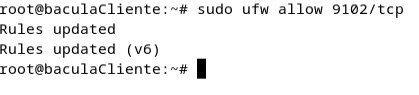
\includegraphics[width=0.5\linewidth]{instalacionBacula/9102alfirewall.png}
    \caption{Adición del puerto 9102 al firewall para permitir la comunicación del File Daemon}
\end{figure}

\textbf{Instalación del Cliente Bacula}
\medskip

Procedemos a instalar el cliente Bacula en el sistema. Este proceso instala todos los componentes necesarios para que el cliente pueda comunicarse con el Director de Bacula.

\begin{verbatim}
apt install bacula-client
\end{verbatim}

A continuación, verificamos que la instalación se ha completado correctamente y que el servicio está activo y ejecutándose.

\begin{figure}[H]
    \centering
    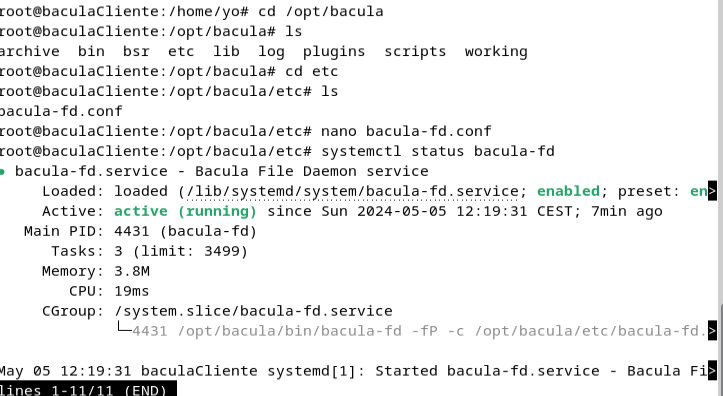
\includegraphics[width=0.5\linewidth]{instalacionBacula/baculaClienteinstalacion2.png}
    \caption{Confirmación de la instalación y estado del servicio Bacula File Daemon}
\end{figure}

\textbf{Configuración del File Daemon}
\medskip

Editamos el archivo de configuración del File Daemon para establecer la conexión con el Director de Bacula. Aquí especificamos el nombre del Director y la contraseña que permite una conexión segura entre el cliente y el servidor.

\begin{verbatim}
nano /opt/bacula/etc/bacula-fd.conf
\end{verbatim}

Añadimos la configuración del Director, especificando su nombre y contraseña correspondiente. Este paso es crucial para la autenticación y la correcta comunicación entre el cliente y el servidor.

\begin{figure}[H]
    \centering
    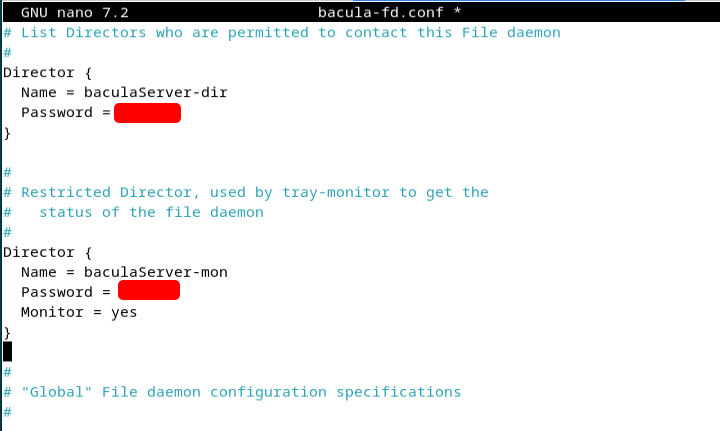
\includegraphics[width=0.5\linewidth]{instalacionBacula/baculaFDcongf.png}
    \caption{Configuración del archivo bacula-fd.conf con detalles del Director}
\end{figure}

Estos pasos garantizan que el cliente Bacula esté correctamente configurado y pueda comunicarse de manera segura con el servidor Bacula Director, facilitando así la gestión centralizada de los respaldos.
